\documentclass{standalone}
\usepackage{tikz}
\usetikzlibrary{patterns, positioning}

\begin{document}
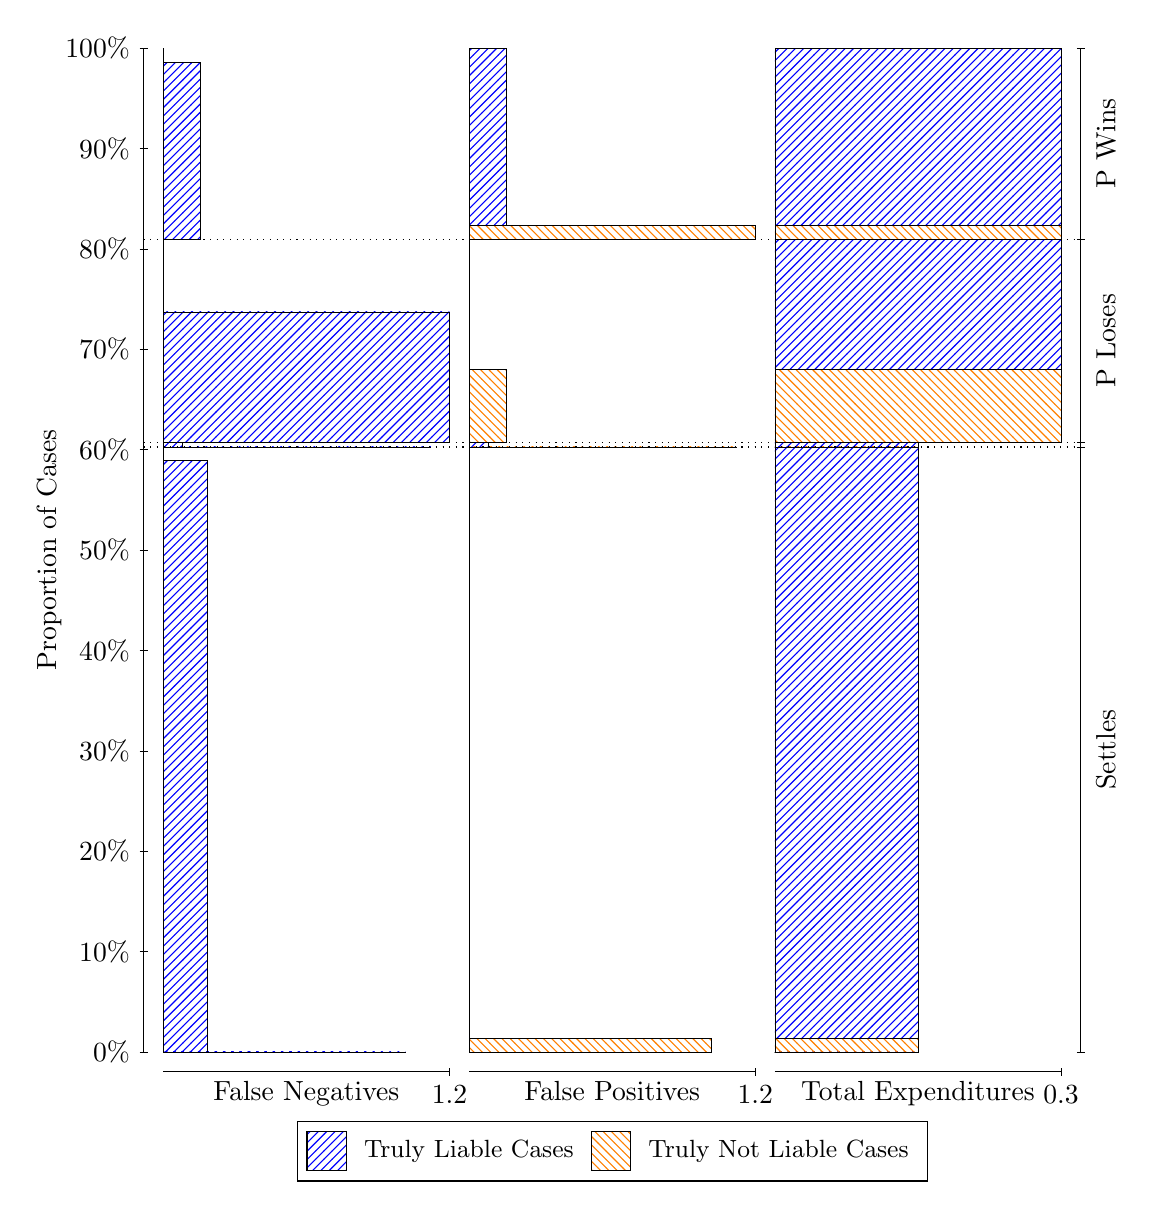
\begin{tikzpicture}
\draw[black, very thin] (1.5,1.75) -- (1.5,14.5);
\node[rotate=90, anchor=center] at (0.3, 8.125) {Proportion of Cases};
\draw[black, very thin] (1.45,1.75) -- (1.55,1.75);
\node[anchor=east] at (1.45, 1.75) {0\%};
\draw[black, very thin] (1.45,3.025) -- (1.55,3.025);
\node[anchor=east] at (1.45, 3.025) {10\%};
\draw[black, very thin] (1.45,4.3) -- (1.55,4.3);
\node[anchor=east] at (1.45, 4.3) {20\%};
\draw[black, very thin] (1.45,5.575) -- (1.55,5.575);
\node[anchor=east] at (1.45, 5.575) {30\%};
\draw[black, very thin] (1.45,6.85) -- (1.55,6.85);
\node[anchor=east] at (1.45, 6.85) {40\%};
\draw[black, very thin] (1.45,8.125) -- (1.55,8.125);
\node[anchor=east] at (1.45, 8.125) {50\%};
\draw[black, very thin] (1.45,9.4) -- (1.55,9.4);
\node[anchor=east] at (1.45, 9.4) {60\%};
\draw[black, very thin] (1.45,10.675) -- (1.55,10.675);
\node[anchor=east] at (1.45, 10.675) {70\%};
\draw[black, very thin] (1.45,11.95) -- (1.55,11.95);
\node[anchor=east] at (1.45, 11.95) {80\%};
\draw[black, very thin] (1.45,13.225) -- (1.55,13.225);
\node[anchor=east] at (1.45, 13.225) {90\%};
\draw[black, very thin] (1.45,14.5) -- (1.55,14.5);
\node[anchor=east] at (1.45, 14.5) {100\%};

\draw[black, very thin] (13.4,1.75) -- (13.4,14.5);
\draw[black, very thin] (13.35,1.75) -- (13.45,1.75);
\node[anchor=west] at (13.35, 1.75) {};
\draw[black, very thin] (13.35,9.4336) -- (13.45,9.4336);
\node[anchor=west] at (13.35, 9.4336) {};
\draw[black, very thin] (13.35,9.4336) -- (13.45,9.4336);
\node[anchor=west] at (13.35, 9.4336) {};
\draw[black, very thin] (13.35,9.4955) -- (13.45,9.4955);
\node[anchor=west] at (13.35, 9.4955) {};
\draw[black, very thin] (13.35,12.07) -- (13.45,12.07);
\node[anchor=west] at (13.35, 12.07) {};
\draw[black, very thin] (13.35,14.5) -- (13.45,14.5);
\node[anchor=west] at (13.35, 14.5) {};

\draw[black, very thin, pattern color=blue, pattern=north east lines] (1.75,1.75) rectangle (4.8304,1.75);
\draw[black, very thin, pattern color=blue, pattern=north east lines] (1.75,1.75) rectangle (4.5145,1.75);
\draw[black, very thin, pattern color=blue, pattern=north east lines] (1.75,1.75) rectangle (4.1986,1.75);
\draw[black, very thin, pattern color=blue, pattern=north east lines] (1.75,1.75) rectangle (3.8826,1.75);
\draw[black, very thin, pattern color=blue, pattern=north east lines] (1.75,1.75) rectangle (3.5667,1.75);
\draw[black, very thin, pattern color=blue, pattern=north east lines] (1.75,1.75) rectangle (3.2507,1.75);
\draw[black, very thin, pattern color=blue, pattern=north east lines] (1.75,1.75) rectangle (2.9348,1.75);
\draw[black, very thin, pattern color=blue, pattern=north east lines] (1.75,1.75) rectangle (2.6188,1.75);
\draw[black, very thin, pattern color=blue, pattern=north east lines] (1.75,1.75) rectangle (2.3029,9.2607);
\draw[black, very thin, pattern color=orange, pattern=north west lines] (1.75,9.2607) rectangle (1.75,9.4336);
\draw[black, very thin, pattern color=blue, pattern=north east lines] (1.75,9.4336) rectangle (5.1464,9.4336);
\draw[black, very thin, pattern color=orange, pattern=north west lines] (1.75,9.4336) rectangle (1.75,9.4336);
\draw[black, very thin, pattern color=blue, pattern=north east lines] (1.75,9.4336) rectangle (1.987,9.4935);
\draw[black, very thin, pattern color=orange, pattern=north west lines] (1.75,9.4935) rectangle (1.75,9.4955);
\draw[black, very thin, pattern color=blue, pattern=north east lines] (1.75,9.4955) rectangle (5.3833,11.15);
\draw[black, very thin, pattern color=orange, pattern=north west lines] (1.75,11.15) rectangle (1.75,12.07);
\draw[black, very thin, pattern color=blue, pattern=north east lines] (1.75,12.07) rectangle (2.2239,14.32);
\draw[black, very thin, pattern color=orange, pattern=north west lines] (1.75,14.32) rectangle (1.75,14.5);
\draw[black, very thin, pattern color=orange, pattern=north west lines] (5.6333,1.75) rectangle (8.7138,1.9229);
\draw[black, very thin, pattern color=orange, pattern=north west lines] (5.6333,1.9229) rectangle (8.3978,1.9229);
\draw[black, very thin, pattern color=orange, pattern=north west lines] (5.6333,1.9229) rectangle (8.0819,1.9229);
\draw[black, very thin, pattern color=orange, pattern=north west lines] (5.6333,1.9229) rectangle (7.7659,1.9229);
\draw[black, very thin, pattern color=orange, pattern=north west lines] (5.6333,1.9229) rectangle (7.45,1.9229);
\draw[black, very thin, pattern color=orange, pattern=north west lines] (5.6333,1.9229) rectangle (7.1341,1.9229);
\draw[black, very thin, pattern color=orange, pattern=north west lines] (5.6333,1.9229) rectangle (7.1341,1.9229);
\draw[black, very thin, pattern color=orange, pattern=north west lines] (5.6333,1.9229) rectangle (6.8181,1.9229);
\draw[black, very thin, pattern color=orange, pattern=north west lines] (5.6333,1.9229) rectangle (6.5022,1.9229);
\draw[black, very thin, pattern color=orange, pattern=north west lines] (5.6333,1.9229) rectangle (6.1862,1.9229);
\draw[black, very thin, pattern color=blue, pattern=north east lines] (5.6333,1.9229) rectangle (5.6333,9.4336);
\draw[black, very thin, pattern color=orange, pattern=north west lines] (5.6333,9.4336) rectangle (5.8703,9.4336);
\draw[black, very thin, pattern color=blue, pattern=north east lines] (5.6333,9.4336) rectangle (5.6333,9.4336);
\draw[black, very thin, pattern color=orange, pattern=north west lines] (5.6333,9.4336) rectangle (9.0297,9.4356);
\draw[black, very thin, pattern color=blue, pattern=north east lines] (5.6333,9.4356) rectangle (5.8703,9.4955);
\draw[black, very thin, pattern color=orange, pattern=north west lines] (5.6333,9.4955) rectangle (6.1072,10.415);
\draw[black, very thin, pattern color=blue, pattern=north east lines] (5.6333,10.415) rectangle (5.6333,12.07);
\draw[black, very thin, pattern color=orange, pattern=north west lines] (5.6333,12.07) rectangle (9.2667,12.25);
\draw[black, very thin, pattern color=blue, pattern=north east lines] (5.6333,12.25) rectangle (6.1072,14.5);
\draw[black, very thin, pattern color=orange, pattern=north west lines] (9.5167,1.75) rectangle (11.333,1.75);
\draw[black, very thin, pattern color=blue, pattern=north east lines] (9.5167,1.75) rectangle (11.333,1.75);
\draw[black, very thin, pattern color=orange, pattern=north west lines] (9.5167,1.75) rectangle (11.333,1.75);
\draw[black, very thin, pattern color=blue, pattern=north east lines] (9.5167,1.75) rectangle (11.333,1.75);
\draw[black, very thin, pattern color=orange, pattern=north west lines] (9.5167,1.75) rectangle (11.333,1.9229);
\draw[black, very thin, pattern color=blue, pattern=north east lines] (9.5167,1.9229) rectangle (11.333,9.4336);
\draw[black, very thin, pattern color=orange, pattern=north west lines] (9.5167,9.4336) rectangle (11.333,9.4336);
\draw[black, very thin, pattern color=blue, pattern=north east lines] (9.5167,9.4336) rectangle (11.333,9.4336);
\draw[black, very thin, pattern color=orange, pattern=north west lines] (9.5167,9.4336) rectangle (11.333,9.4356);
\draw[black, very thin, pattern color=blue, pattern=north east lines] (9.5167,9.4356) rectangle (11.333,9.4955);
\draw[black, very thin, pattern color=orange, pattern=north west lines] (9.5167,9.4955) rectangle (13.15,10.415);
\draw[black, very thin, pattern color=blue, pattern=north east lines] (9.5167,10.415) rectangle (13.15,12.07);
\draw[black, very thin, pattern color=orange, pattern=north west lines] (9.5167,12.07) rectangle (13.15,12.25);
\draw[black, very thin, pattern color=blue, pattern=north east lines] (9.5167,12.25) rectangle (13.15,14.5);
\draw[black, dotted] (1.5,9.4336) -- (13.4,9.4336);
\draw[black, dotted] (1.5,9.4336) -- (13.4,9.4336);
\draw[black, dotted] (1.5,9.4955) -- (13.4,9.4955);
\draw[black, dotted] (1.5,12.07) -- (13.4,12.07);
\draw[black, very thin] (1.75,1.5) -- (5.3833,1.5);
\node[anchor=north] at (3.5667, 1.5) {False Negatives};
\draw[black, very thin] (5.3833,1.45) -- (5.3833,1.55);
\node[anchor=north] at (5.3833, 1.45) {1.2};

\draw[black, very thin] (5.6333,1.5) -- (9.2667,1.5);
\node[anchor=north] at (7.45, 1.5) {False Positives};
\draw[black, very thin] (9.2667,1.45) -- (9.2667,1.55);
\node[anchor=north] at (9.2667, 1.45) {1.2};

\draw[black, very thin] (9.5167,1.5) -- (13.15,1.5);
\node[anchor=north] at (11.333, 1.5) {Total Expenditures};
\draw[black, very thin] (13.15,1.45) -- (13.15,1.55);
\node[anchor=north] at (13.15, 1.45) {0.3};

\node[black, centered, rotate=90] at (13.72, 5.5918) {Settles};


\node[black, centered, rotate=90] at (13.72, 10.783) {P Loses};
\node[black, centered, rotate=90] at (13.72, 13.285) {P Wins};

\draw (7.449999999999999,1.5) node[draw=none] (baseCoordinate) {};
\begin{scope}[align=center]
        \matrix[scale=0.5, draw=black, below=0.5cm of baseCoordinate, nodes={draw}, column sep=0.1cm]{
            \node[rectangle, draw, minimum width=0.5cm, minimum height=0.5cm, pattern=north east lines, pattern color=blue] {}; &
            \node[draw=none, font=\small] (B) {Truly Liable Cases}; &
            \node[rectangle, draw, minimum width=0.5cm, minimum height=0.5cm, pattern=north west lines, pattern color=orange] {}; &
            \node[draw=none, font=\small] (B) {Truly Not Liable Cases}; \\
            };
\end{scope}

\end{tikzpicture}
\end{document}